%& C:\Users\RANGAR~1\AppData\Roaming\TikzEdt\TikzEdt\023~1.0\TEMP_H~1
\begin{document}
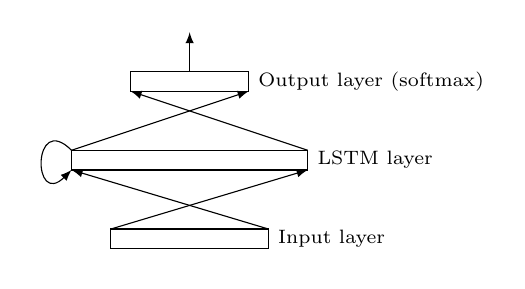
\begin{tikzpicture}[x=0.5cm, y=0.5cm, every node/.append style={text=black, font=\scriptsize}]
	\draw  (0,0) -- ++(2, 0) -- ++(0, 0.5) coordinate  (a)  node [midway, anchor=west] {Input layer} -- ++(-4, 0) coordinate  (b) -- ++(0, -0.5) -- cycle;
	
	
	\draw  (0,2) -- ++(3, 0) coordinate  (c) -- ++(0, 0.5) coordinate (d) node [midway, anchor=west] {LSTM layer}  -- ++(-6, 0) coordinate  (e) -- ++(0, -0.5)  coordinate  (f)  -- cycle;
	
	\draw  (0,4) -- ++(1.5, 0)  coordinate  (g) -- ++(0, 0.5) node [midway, anchor=west] {Output layer (softmax)}  -- ++(-3, 0) coordinate[midway] (t) -- ++(0, -0.5) coordinate  (h) -- cycle;	
	
	\draw[-latex] (a) -- (f);
	\draw[-latex] (b) -- (c);
	
	\draw[-latex] (e) -- (g);
	\draw[-latex] (d) -- (h);	
	
	\draw[-latex] (t) -- ++(0, 1);		
	\draw[-latex] (e)  .. controls ++(-1,1) and ++(-1, -1) ..  (f);

\usetikzlibrary{calc}
\pgftransformreset
\node[inner sep=0pt,outer sep=0pt,minimum size=0pt,line width=0pt,text width=0pt,text height=0pt] at (current bounding box) {};
%add border to avoid cropping by pdflibnet
\foreach \border in {0.1}
  \useasboundingbox (current bounding box.south west)+(-\border,-\border) rectangle (current bounding box.north east)+(\border,\border);
\newwrite\metadatafile
\immediate\openout\metadatafile=\jobname_BB.txt
\path
  let
    \p1=(current bounding box.south west),
    \p2=(current bounding box.north east)
  in
  node[inner sep=0pt,outer sep=0pt,minimum size=0pt,line width=0pt,text width=0pt,text height=0pt,draw=white] at (current bounding box) {
\immediate\write\metadatafile{\p1,\p2}
};
\immediate\closeout\metadatafile
\end{tikzpicture}

\end{document}
